\documentclass{article}
\usepackage[utf8]{inputenc}
\usepackage[spanish]{babel}
\usepackage{listings}
\usepackage{graphicx}
\graphicspath{ {imagenes/} }
\usepackage{cite}

\begin{document}

\begin{titlepage}
    \begin{center}
        \vspace*{1cm}
            
        \Huge
        \textbf{Memorias de un computador}
            
        \vspace{0.5cm}
            
        \vspace{1.5cm}
            
        \textbf{Andrés Felipe Giraldo Yusti}
            
        \vfill
            
        \vspace{0.8cm}
            
        \Large
        Despartamento de Ingeniería Electrónica y Telecomunicaciones\\
        Universidad de Antioquia\\
        Medellín\\
        Septiembre de 2020
            
    \end{center}
\end{titlepage}

\tableofcontents

\section{Introducción}
La memoria del computador es la parte mas importante para que este pueda funcionar, es la que decide la cantidad de datos a menar y a la velocidad que lo hará el computador y a continuacion hablaremos de estas, como funcionan y su importancia

\section{Que es la memoria del computador} \label{Que es la memoria del computador}


Se considera memoria a todo tipo de dispositivo de almacenamiento electrónico, usualmente se utiliza el término para referirse a dispositivos de almacenamiento temporal y alta velocidad de acceso, como lo es la memoria principal del computador.\cite{knuth-fa}

\vspace{0.5cm}

La memoria del computador son dispositivos donde se guardan los datos para que los procesadores puedan trabajarlos y así devolverles a los usuarios los resultados que necesitan. estas memorias pueden guardar los datos permanentemente como un disco duro donde la informacion se queda guardada aunque el computador se apague y tambien se guardan los datos temporalmente como la memoria ram donde elimina los datos que no esta usando para abrir espacio y asi trabajar con informacion distinta.
\clearpage

\section{Tipos de memorias} \label{Tipos de memorias}

\subsection{Memoria RAM}

\begin{figure}[h]
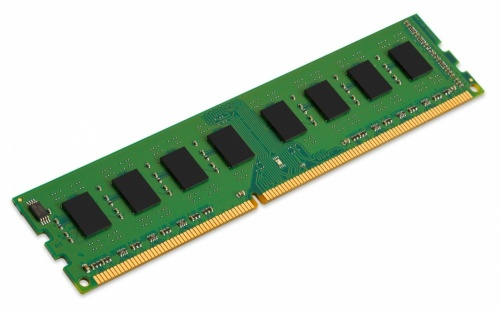
\includegraphics[width=5cm]{RAM.jpg}
\centering
\caption{RAM}
\label{fig:RAM}
\end{figure}
Random Access Memory, es una memoria de lectura y escritura, tambien es una memoria de almacenamiento tamporal donde se guardan datos que se estan usando y son eliminados cuando el procesador ya no los necesita.

\vspace{0.5cm}

Hay dos tipos de memoria RAM, la memoria RAM dinamica (DRAM) y la memoria RAM estatica (SRAM).

\subsection{memoria caché}
En informática, se conoce como memoria caché o memoria de acceso rápido a uno de los recursos con los que cuenta una CPU (Central Processing Unit, o sea, Unidad Central de Procesamiento) para almacenar temporalmente los datos recientemente procesados en un búfer especial, es decir, en una memoria auxiliar.\cite{pagina} Esta memoria es mas cara que la RAM y tiene menos almacenamiento, pero es más rapida. 


\begin{figure}[h]
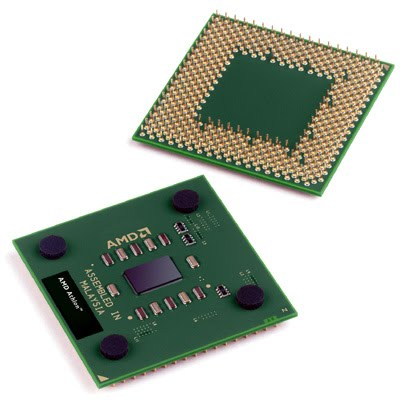
\includegraphics[width=5cm]{CACHE.jpg}
\centering
\caption{Memoria caché}
\label{fig:RAM}
\end{figure}


\subsection{Memoria rom}

\begin{figure}[h]
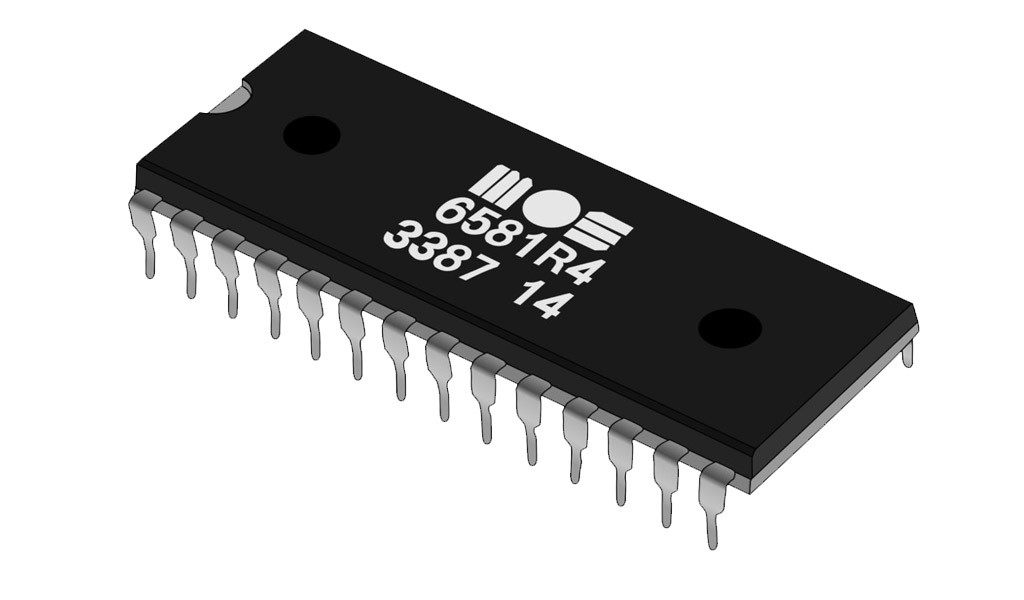
\includegraphics[width=5cm]{ROM.jpg}
\centering
\caption{ROM}
\label{fig:RAM}
\end{figure}

Read Only Memory,es un tipo de memoria que es solo de lectura, es decir, que no se puede modificar ya que no se puede escribir en ella, se encuentra en la placa base y su funcion es dar inicio a la bios para poder encender y hacer funcionar el computador.\cite{pagina2}

\subsection{Memoria Flash}

\begin{figure}[h]
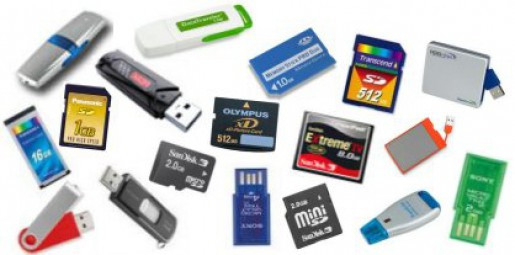
\includegraphics[width=5cm]{FLASH.jpg}
\centering
\caption{Memoria Flash}
\label{fig:RAM}
\end{figure}

Son dispositivos de almacenamiento portatil con la capacidad de guardar grandes cantidades de datos y son memoras de lectura y escritura que, a diferencia de la memoria RAM, estas no son memorias volatiles ya que guardan los datos aunque no se esten usando.
\clearpage

\subsection{VRAM}

\begin{figure}[h]
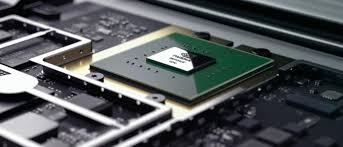
\includegraphics[width=5cm]{VRAM.jpg}
\centering
\caption{VRAM}
\label{fig:RAM}
\end{figure}

Es un tipo de memoria que se encuentra en todas las tarjetas graficas y es una memoria que es usada solo en tareas especificas como por ejemplo aplicaciones graficas o videojuegos

\subsection{Memoria virtual}
Esta sirve para guardar pequeñas porciones de un programa que no se estan usando, pero que despues se usaran

\section{Como se gestiona la memoria en un computador} \label{Como se gestiona la memoria en un computador}

Un computador necesita de varias memorias para que este pueda funcionar, ya que estas cumplen diferentes funciones y el computador las ocupa así:
\vspace{0.5cm}

Saca los datos del disco duro y los manda a la memoria RAM (no mandara todos los datos de la aplicación sino los datos específicos que está usando en ese instante) donde trabajará el procesador para mandarle los datos que necesita al usuario, cuando el usuario ya no esté usando esa aplicación, automáticamente la memoria RAM eliminara los datos que guardó anteriormente.
\vspace{0.5cm}

Si el usuario desea guardar esa información, devolverá los datos al disco duro donde estarán seguros.


\section{¿Qué hace que una memoria sea más rápida que otra? ¿Por qué esto es importante?} \label{¿Qué hace que una memoria sea más rápida que otra? ¿Por qué esto es importante?}

Como sabemos, la frecuencia de la memoria RAM se basa en ciclos de reloj. Cada lectura y escritura que se hacen en ella representa un ciclo y por lo tanto su rendimiento se mide en cantidad de ciclos por segundo que puede realizar. Un ejemplo sencillo sería decir que una memoria a 2.133 MHz realiza 2,1 billones de ciclos por segundo.\cite{pagina3}
\vspace{0.5cm}

Y es importante porque entre mas veloz sea, mas datos puede leer y almacenar por segundo y menos tiempo le consumirá al usuario al momento de realizar una tarea

\section{Conclusión} \label{conclulsion}
La memoria es una parte vital del pc y de ella depente la eficiencia de estos, tambien la cantidad de datos que puede guardar y usar en un momento determinado. sin ella no seria posible la funcionalidad del computador, ya que no tendriamos datos que manipular o procesar.

\bibliographystyle{IEEEtran}
\bibliography{references}

\end{document}
